% Created by tikzDevice version 0.10.1 on 2016-08-25 15:47:44
% !TEX encoding = UTF-8 Unicode
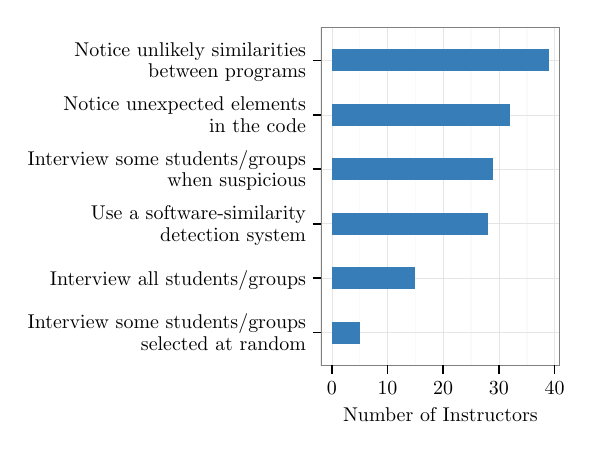
\begin{tikzpicture}[x=1pt,y=1pt]
\definecolor{fillColor}{RGB}{255,255,255}
\path[use as bounding box,fill=fillColor,fill opacity=0.00] (0,0) rectangle (195.13,144.54);
\begin{scope}
\path[clip] (  0.00,  0.00) rectangle (195.13,144.54);
\definecolor{drawColor}{RGB}{255,255,255}
\definecolor{fillColor}{RGB}{255,255,255}

\path[draw=drawColor,line width= 0.6pt,line join=round,line cap=round,fill=fillColor] (  0.00,  0.00) rectangle (195.13,144.54);
\end{scope}
\begin{scope}
\path[clip] (105.98, 22.52) rectangle (192.28,144.54);
\definecolor{fillColor}{RGB}{255,255,255}

\path[fill=fillColor] (105.98, 22.52) rectangle (192.28,144.54);
\definecolor{drawColor}{gray}{0.98}

\path[draw=drawColor,line width= 0.6pt,line join=round] (119.96, 22.52) --
	(119.96,144.54);

\path[draw=drawColor,line width= 0.6pt,line join=round] (140.08, 22.52) --
	(140.08,144.54);

\path[draw=drawColor,line width= 0.6pt,line join=round] (160.19, 22.52) --
	(160.19,144.54);

\path[draw=drawColor,line width= 0.6pt,line join=round] (180.31, 22.52) --
	(180.31,144.54);
\definecolor{drawColor}{gray}{0.90}

\path[draw=drawColor,line width= 0.2pt,line join=round] (105.98, 34.33) --
	(192.28, 34.33);

\path[draw=drawColor,line width= 0.2pt,line join=round] (105.98, 54.01) --
	(192.28, 54.01);

\path[draw=drawColor,line width= 0.2pt,line join=round] (105.98, 73.69) --
	(192.28, 73.69);

\path[draw=drawColor,line width= 0.2pt,line join=round] (105.98, 93.37) --
	(192.28, 93.37);

\path[draw=drawColor,line width= 0.2pt,line join=round] (105.98,113.05) --
	(192.28,113.05);

\path[draw=drawColor,line width= 0.2pt,line join=round] (105.98,132.73) --
	(192.28,132.73);

\path[draw=drawColor,line width= 0.2pt,line join=round] (109.90, 22.52) --
	(109.90,144.54);

\path[draw=drawColor,line width= 0.2pt,line join=round] (130.02, 22.52) --
	(130.02,144.54);

\path[draw=drawColor,line width= 0.2pt,line join=round] (150.14, 22.52) --
	(150.14,144.54);

\path[draw=drawColor,line width= 0.2pt,line join=round] (170.25, 22.52) --
	(170.25,144.54);

\path[draw=drawColor,line width= 0.2pt,line join=round] (190.37, 22.52) --
	(190.37,144.54);
\definecolor{fillColor}{RGB}{55,126,184}

\path[fill=fillColor] (109.90, 30.39) rectangle (119.96, 38.26);

\path[fill=fillColor] (109.90, 50.07) rectangle (140.08, 57.94);

\path[fill=fillColor] (109.90, 69.75) rectangle (166.23, 77.62);

\path[fill=fillColor] (109.90, 89.43) rectangle (168.24, 97.31);

\path[fill=fillColor] (109.90,109.11) rectangle (174.28,116.99);

\path[fill=fillColor] (109.90,128.80) rectangle (188.36,136.67);
\definecolor{drawColor}{gray}{0.50}

\path[draw=drawColor,line width= 0.6pt,line join=round,line cap=round] (105.98, 22.52) rectangle (192.28,144.54);
\end{scope}
\begin{scope}
\path[clip] (  0.00,  0.00) rectangle (195.13,144.54);
\definecolor{drawColor}{RGB}{0,0,0}

\node[text=drawColor,anchor=base east,inner sep=0pt, outer sep=0pt, scale=  0.72] at (100.58, 35.73) {Interview some students/groups};

\node[text=drawColor,anchor=base east,inner sep=0pt, outer sep=0pt, scale=  0.72] at (100.58, 27.96) {selected at random};

\node[text=drawColor,anchor=base east,inner sep=0pt, outer sep=0pt, scale=  0.72] at (100.58, 51.53) {Interview all students/groups};

\node[text=drawColor,anchor=base east,inner sep=0pt, outer sep=0pt, scale=  0.72] at (100.58, 75.10) {Use a software-similarity};

\node[text=drawColor,anchor=base east,inner sep=0pt, outer sep=0pt, scale=  0.72] at (100.58, 67.32) {detection system};

\node[text=drawColor,anchor=base east,inner sep=0pt, outer sep=0pt, scale=  0.72] at (100.58, 94.78) {Interview some students/groups};

\node[text=drawColor,anchor=base east,inner sep=0pt, outer sep=0pt, scale=  0.72] at (100.58, 87.00) {when suspicious};

\node[text=drawColor,anchor=base east,inner sep=0pt, outer sep=0pt, scale=  0.72] at (100.58,114.46) {Notice unexpected elements};

\node[text=drawColor,anchor=base east,inner sep=0pt, outer sep=0pt, scale=  0.72] at (100.58,106.68) {in the code};

\node[text=drawColor,anchor=base east,inner sep=0pt, outer sep=0pt, scale=  0.72] at (100.58,134.14) {Notice unlikely similarities};

\node[text=drawColor,anchor=base east,inner sep=0pt, outer sep=0pt, scale=  0.72] at (100.58,126.36) {between programs};
\end{scope}
\begin{scope}
\path[clip] (  0.00,  0.00) rectangle (195.13,144.54);
\definecolor{drawColor}{RGB}{0,0,0}

\path[draw=drawColor,line width= 0.6pt,line join=round] (102.98, 34.33) --
	(105.98, 34.33);

\path[draw=drawColor,line width= 0.6pt,line join=round] (102.98, 54.01) --
	(105.98, 54.01);

\path[draw=drawColor,line width= 0.6pt,line join=round] (102.98, 73.69) --
	(105.98, 73.69);

\path[draw=drawColor,line width= 0.6pt,line join=round] (102.98, 93.37) --
	(105.98, 93.37);

\path[draw=drawColor,line width= 0.6pt,line join=round] (102.98,113.05) --
	(105.98,113.05);

\path[draw=drawColor,line width= 0.6pt,line join=round] (102.98,132.73) --
	(105.98,132.73);
\end{scope}
\begin{scope}
\path[clip] (  0.00,  0.00) rectangle (195.13,144.54);
\definecolor{drawColor}{RGB}{0,0,0}

\path[draw=drawColor,line width= 0.6pt,line join=round] (109.90, 19.52) --
	(109.90, 22.52);

\path[draw=drawColor,line width= 0.6pt,line join=round] (130.02, 19.52) --
	(130.02, 22.52);

\path[draw=drawColor,line width= 0.6pt,line join=round] (150.14, 19.52) --
	(150.14, 22.52);

\path[draw=drawColor,line width= 0.6pt,line join=round] (170.25, 19.52) --
	(170.25, 22.52);

\path[draw=drawColor,line width= 0.6pt,line join=round] (190.37, 19.52) --
	(190.37, 22.52);
\end{scope}
\begin{scope}
\path[clip] (  0.00,  0.00) rectangle (195.13,144.54);
\definecolor{drawColor}{RGB}{0,0,0}

\node[text=drawColor,anchor=base,inner sep=0pt, outer sep=0pt, scale=  0.72] at (109.90, 12.16) {0};

\node[text=drawColor,anchor=base,inner sep=0pt, outer sep=0pt, scale=  0.72] at (130.02, 12.16) {10};

\node[text=drawColor,anchor=base,inner sep=0pt, outer sep=0pt, scale=  0.72] at (150.14, 12.16) {20};

\node[text=drawColor,anchor=base,inner sep=0pt, outer sep=0pt, scale=  0.72] at (170.25, 12.16) {30};

\node[text=drawColor,anchor=base,inner sep=0pt, outer sep=0pt, scale=  0.72] at (190.37, 12.16) {40};
\end{scope}
\begin{scope}
\path[clip] (  0.00,  0.00) rectangle (195.13,144.54);
\definecolor{drawColor}{RGB}{0,0,0}

\node[text=drawColor,anchor=base,inner sep=0pt, outer sep=0pt, scale=  0.72] at (149.13,  2.40) {Number of Instructors};
\end{scope}
\end{tikzpicture}
